\documentclass[12pt, titlepage]{article}

\usepackage{fullpage}
\usepackage[round]{natbib}
\usepackage{multirow}
\usepackage{booktabs}
\usepackage{tabularx}
\usepackage{graphicx}
\usepackage{float}
\usepackage{hyperref}
\hypersetup{
    colorlinks,
    citecolor=blue,
    filecolor=black,
    linkcolor=red,
    urlcolor=blue
}

%% Comments

\usepackage{color}

\newif\ifcomments\commentstrue %displays comments
%\newif\ifcomments\commentsfalse %so that comments do not display

\ifcomments
\newcommand{\authornote}[3]{\textcolor{#1}{[#3 ---#2]}}
\newcommand{\todo}[1]{\textcolor{red}{[TODO: #1]}}
\else
\newcommand{\authornote}[3]{}
\newcommand{\todo}[1]{}
\fi

\newcommand{\wss}[1]{\authornote{blue}{SS}{#1}} 
\newcommand{\plt}[1]{\authornote{magenta}{TPLT}{#1}} %For explanation of the template
\newcommand{\an}[1]{\authornote{cyan}{Author}{#1}}

%% Common Parts

\newcommand{\progname}{ProgName} % PUT YOUR PROGRAM NAME HERE
\newcommand{\authname}{Team \#, Team Name
\\ Student 1 name
\\ Student 2 name
\\ Student 3 name
\\ Student 4 name} % AUTHOR NAMES                  

\usepackage{hyperref}
    \hypersetup{colorlinks=true, linkcolor=blue, citecolor=blue, filecolor=blue,
                urlcolor=blue, unicode=false}
    \urlstyle{same}
                                


\newcounter{acnum}
\newcommand{\actheacnum}{AC\theacnum}
\newcommand{\acref}[1]{AC\ref{#1}}

\newcounter{ucnum}
\newcommand{\uctheucnum}{UC\theucnum}
\newcommand{\uref}[1]{UC\ref{#1}}

\newcounter{mnum}
\newcommand{\mthemnum}{M\themnum}
\newcommand{\mref}[1]{M\ref{#1}}

\begin{document}

\title{System Design for \progname{}} 
\author{\authname}
\date{\today}

\maketitle

\pagenumbering{roman}

\section{Revision History}

\begin{tabularx}{\textwidth}{p{3cm}p{2cm}X}
\toprule {\bf Date} & {\bf Version} & {\bf Notes}\\
\midrule
February 18, 2023 & 1.0 & Initial Version\\
\bottomrule
\end{tabularx}

\newpage

\section{Reference Material}

This section records information for easy reference.

\subsection{Abbreviations and Acronyms}

\renewcommand{\arraystretch}{1.2}
\begin{tabular}{l l} 
  \toprule		
  \textbf{symbol} & \textbf{description}\\
  \midrule 
  \progname & The Software Engineering Capstone Project Course at McMaster University\\
  Figma & A collaborative web application for interface design\\
  HTTP / HTTPS & Hypertext Transfer Protocol, a communications protocol for network interactions\\
  Web Socket &  A communications protocol used for two-way interaction\\
  MDN Web Docs & A documentation repository for web developers\\
  AWS &  Amazon Web Services, a cloud computing platform\\
  Angular & A web framework for building web applications.\\
  Node.js & A JavaScript run-time.\\
  MongoDB & A database program.\\
  Google Oauth & An authentication service by Google.\\
  Docker & A container engine.\\
  \bottomrule
\end{tabular}\\

\newpage

\tableofcontents

\newpage

\listoftables

\listoffigures

\newpage

\pagenumbering{arabic}

\section{Introduction}
This document describes the design for the CodeChamp system. The design document is split up into three documents, the \href{https://github.com/Tamas-Leung/CodeChamp/tree/main/docs/Design/MIS}{Module Interface Specification}, \href{https://github.com/Tamas-Leung/CodeChamp/tree/main/docs/Design/MG}{Module Guide} and the system design document. Other relevant documentation is listed below:
\begin{enumerate}
    \item \href{https://github.com/Tamas-Leung/CodeChamp/tree/main/docs/DevelopmentPlan}{Development Plan}
    \item \href{https://github.com/Tamas-Leung/CodeChamp/tree/main/docs/SRS}{System Requirements Specification} 
    \item \href{https://github.com/Tamas-Leung/CodeChamp/blob/main/docs/HazardAnalysis/HazardAnalysis.md}{Hazard Analysis}
    \item \href{https://github.com/Tamas-Leung/CodeChamp/blob/main/docs/VnVPlan}{Validation \& Verification Plan} 
    
\end{enumerate}

\section{Purpose}

This document is written to describe the architecture and the design decisions in the CodeChamp system. Primarily, it introduces the scope of the system to demonstrate the possible interactions with the outside world. Moreover, it gives an overview of the project, recounting the important components from a high level and describing the normal behavior of the system. Additionally, it gives a high-level overview of the event handling mechanisms in place for undesired behavior. Since the CodeChamp system is user-centric, the document also describes mock-ups for the user interface design of the system. Finally, a timeline is given for the implementation of the system. 


\section{Scope}


\begin{figure}[H]
\centering
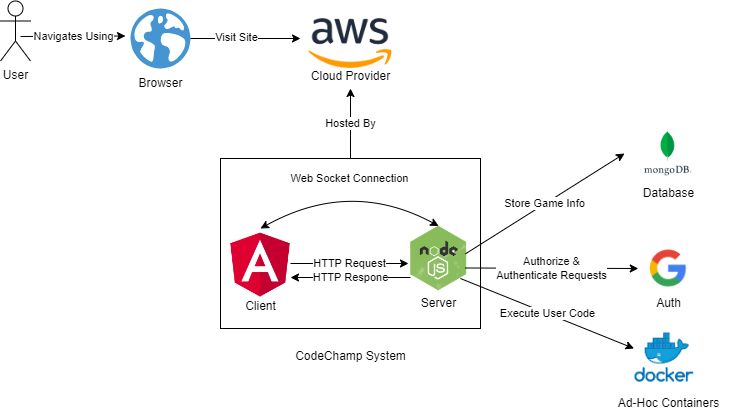
\includegraphics[scale=0.65]{Design/SystDesign/SystemBoundary.png}
\caption{Context Diagram for the CodeChamp System}
\end{figure}

\section{Project Overview}

\subsection{Normal Behaviour}
The CodeChamp system is seperated into an Angular front-end and a Node.js backend. Normally, the user will access the front-end throw a web browser on a desktop application. The client will send network requests using HTTPS to the back-end and successfully receive a response. For parts of the application which require bidirectional connectivity, such as live updates during a game or in the lobby, a WebSocket connection will be used. Additionally, the CodeChamp system will interact with various external services. For storing and retrieving items from the database, a MongoDB cluster will be used. When needed, the backend will query MongoDB to retrieve and/or store an object when a client requests it. Furthermore, for authentication purposes, such as for signing in users, Google Oauth will be queried. Finally, when a user submits code to be executed, a docker container will be created to execute and evaluate the submission.

The following user journey specifies the average expected experience for a user of the CodeChamp system:
\begin{enumerate}
    \item User navigates to the site using web browser
    \item User logs into the application
    \item User creates/joins a game
    \item The game starts once the lobby is ready
    \item User plays the game by attempting to solve the problem
    \item User proceeds to the next round upon successfully completing a round
    \item User loses after being unable to complete a round / user wins by winning all the rounds
    \item User checks their personal statistics and match history by going to the Home Page and clicking on the personal profile button
    \item User checks the leaderboard by going to the Home Page and clicking on the leaderboard button
\end{enumerate}

\subsection{Undesired Event Handling}
Exceptions which occur in the Backend APIs will be propagated as HTTP status codes. The engineers will ensure to follow the conventions established in the \href{https://developer.mozilla.org/en-US/docs/Web/HTTP/Status}{MDN Web Docs} in order to distinguish client error responses and server error responses. Furthermore, internal server errors will be logged and will be made accessible for developers through the AWS portal in production. This ensures that developers can quickly identify and debug issues that arise. The front-end will use the Angular error interceptor in order to detect error responses and will forward them to the pages to handle accordingly. In the case of errors, the front-end will display a dialog mentioning the event in natural language to the user and suggesting an solution. For example, for client errors, this may be to take a different action. For internal server errors, it may suggest for them to retry the action at a different time. Additionally, errors occurring on the front-end will also be made accessible for developers through the AWS portal in production .

\subsection{Component Diagram}

\begin{figure}[H]
\centering
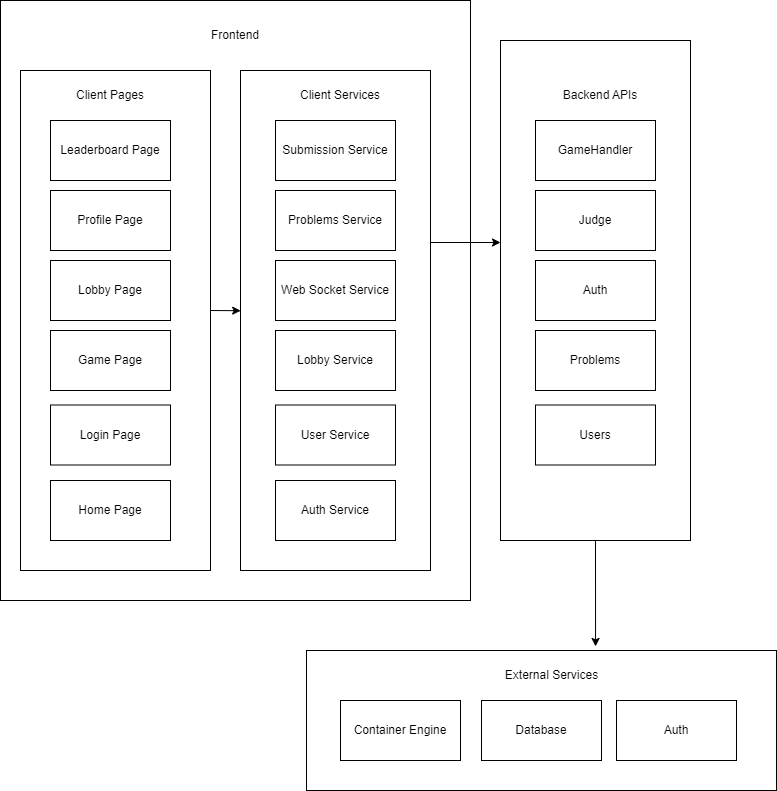
\includegraphics[width=0.8\textwidth]{Design/SystDesign/ComponentDiagram.png}
\caption{Component Diagram for the CodeChamp System}
\end{figure}

\subsection{Connection Between Requirements and Design} \label{SecConnection}

\begin{table}[H]
\centering 
\begin{tabular}{p{0.2\textwidth} p{0.6\textwidth}}
\toprule
\textbf{Req.} & \textbf{Decisions}\\
\midrule
NFR11 & Users use username, password and email to create accounts. Google Oauth is used as part of the implementation.\\ 
FR6, FR14, FR15 & Using Docker as the containerized engine to run and compile code to avoid the effects of running malicious code.\\
FR3 & Game cuts player count in half in each round to have at most 4 rounds.\\
FR.23 & Using unique yet human readable IDs/lobby codes for ease of joining. \\
FR.13 & The system allows developers to create/modify tests through network calls. \\
FR.1 & System uses random matchmaking instead of the other option, skill based match making. \\
\hline
\end{tabular}
\caption{Requirements and Design Decisions made}
\label{TblRT2}
\end{table}

% \wss{The intention of this section is to document decisions that are made
%   ``between'' the requirements and the design.  To satisfy some requirements,
%   design decisions need to be made.  Rather than make these decisions implicit,
%   they are explicitly recorded here.  For instance, if a program has security
%   requirements, a specific design decision may be made to satisfy those
%   requirements with a password.}

\section{User Interfaces}

The following mock-ups were produced using Figma for the CodeChamp user interface: 

\begin{figure}[H]
\centering
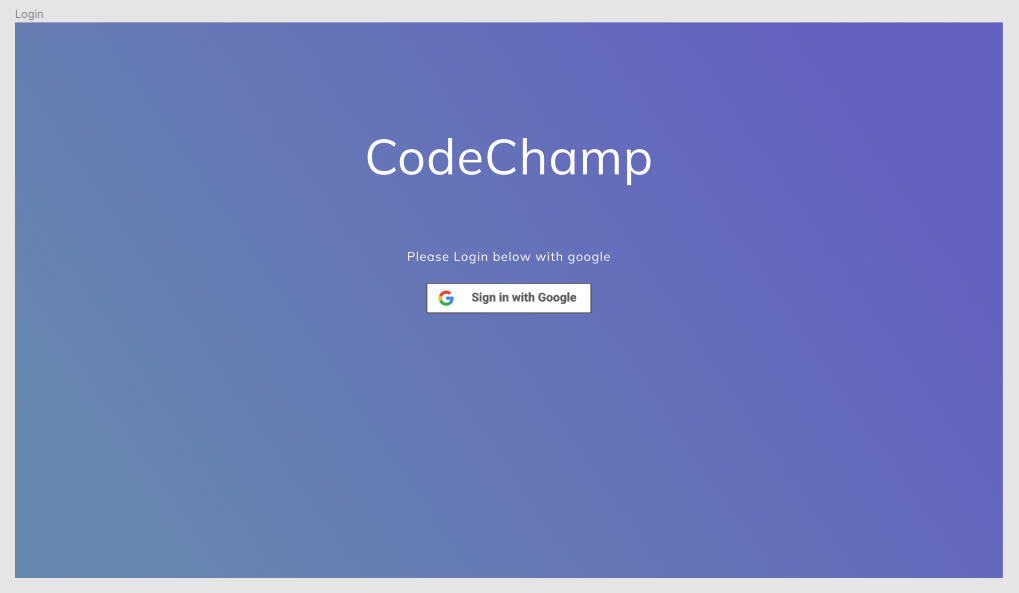
\includegraphics[width=0.8\textwidth]{Design/SystDesign/LoginPage.png}
\caption{Mock-up for CodeChamp's Login Page}
\end{figure}

\begin{figure}[H]
\centering
\includegraphics[width=0.8\textwidth]{Design/SystDesign/HomePage.png}
\caption{Mock-up for CodeChamp's Home Page}
\end{figure}

\begin{figure}[H]
\centering
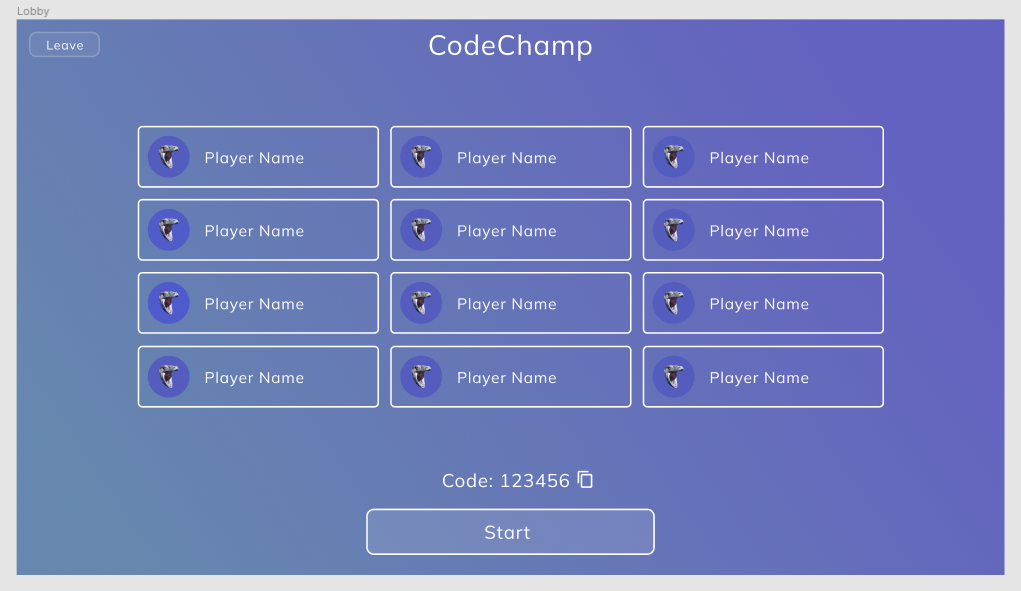
\includegraphics[width=0.8\textwidth]{Design/SystDesign/LobbyPage.png}
\caption{Mock-up for CodeChamp's Lobby Page}
\end{figure}

\begin{figure}[H]
\centering
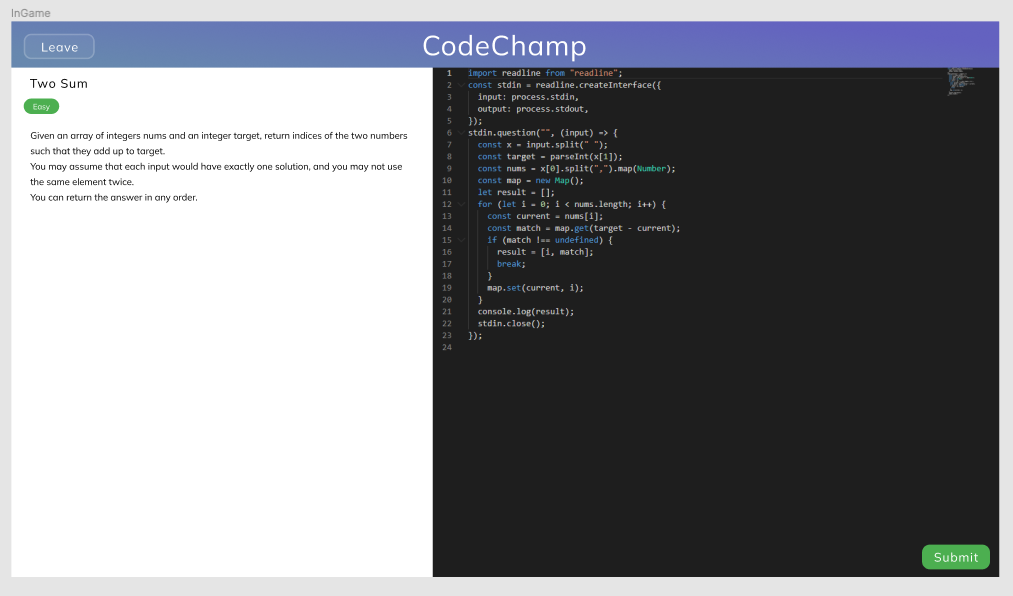
\includegraphics[width=0.8\textwidth]{Design/SystDesign/GamePage.png}
\caption{Mock-up for CodeChamp's Game Page}
\end{figure}

\begin{figure}[H]
\centering
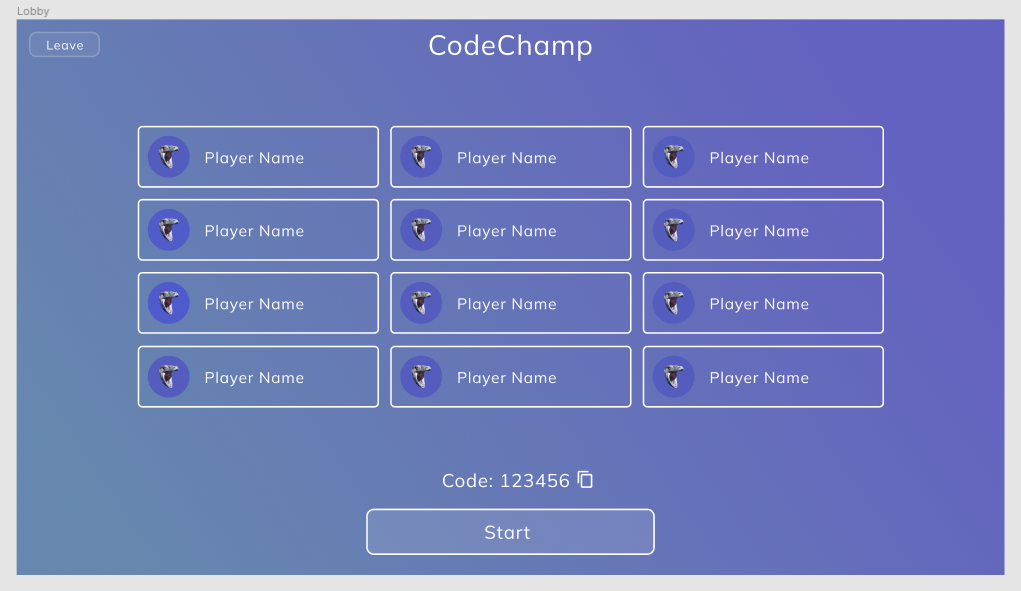
\includegraphics[width=0.8\textwidth]{Design/SystDesign/LeaderboardPage.png}
\caption{Mock-up for CodeChamp's Leaderboard Page}
\end{figure}

\begin{figure}[H]
\centering
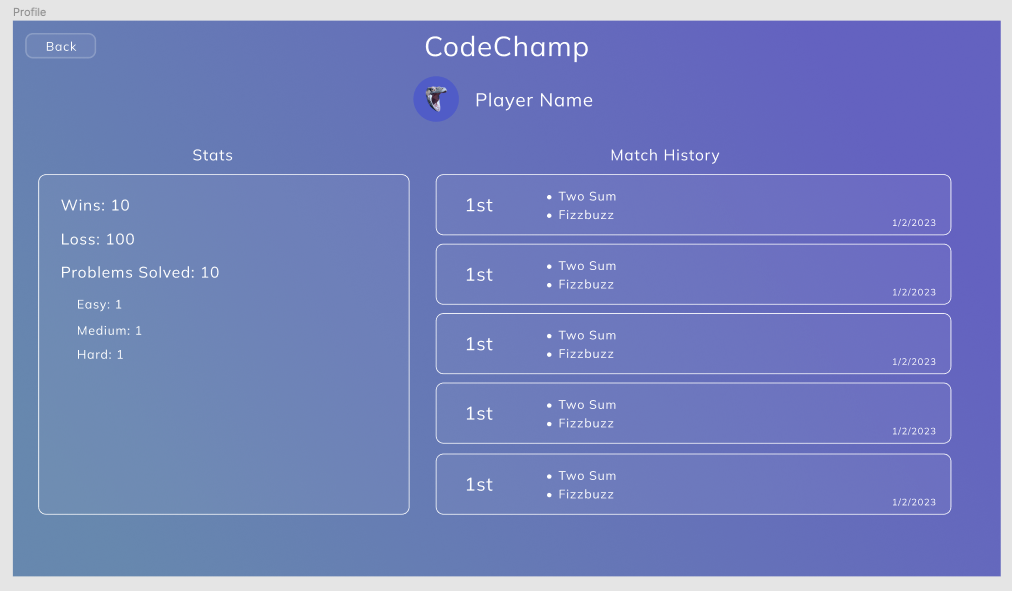
\includegraphics[width=0.8\textwidth]{Design/SystDesign/ProfilePage.png}
\caption{Mock-up for CodeChamp's Profile Page}
\end{figure}

\begin{figure}[H]
\centering
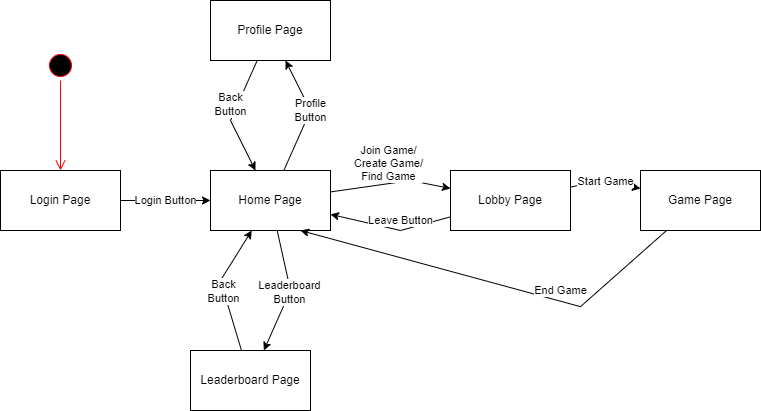
\includegraphics[width=1\textwidth]{Design/SystDesign/State.png}
\caption{State Machine for front end pages}
\end{figure}

\section{Design of Hardware}

N/A

\section{Design of Electrical Components}

N/A

\section{Design of Communication Protocols}

HTTPS is utilized to send requests from the front-end and retrieve data from the servers and database. For bi-directional messaging between clients and servers, WebSocket technology is used. These are standard technologies and are not implemented by the CodeChamp team.

\section{Timeline}


\begin{table}[H]
\centering
\begin{tabular}{p{0.35\textwidth} p{0.3\textwidth}  p{0.3\textwidth}}
\toprule
Module & Completion By Date & Responsible Engineer(s) \\
\midrule
ClientT Module & 2022-12-30 & Anton\\
GameT Module & 2022-12-30 & Anton\\
MatchT Module & 2023-02-11 & Zhiming\\
UserT Module & 2023-02-11 & Zhiming\\
UserStatsT Module & 2023-02-11 & Zhiming\\
ProblemT Module & 2022-11-14 & Tamas\\ 
Difficulty Module & 2022-11-14 & Tamas\\
TestCaseT Module & 2022-11-14 & Youssef\\
SubmissionT Module & 2022-11-14 & Youssef\\
JudgeResultT Module & 2022-11-14 & Youssef\\
JudgeVerdict Module & 2022-11-14 & Youssef\\
TestCaseVerdictT Module & 2022-11-14 & Youssef\\
HomePage Module & 2023-1-21 & Zhiming, Dipendra\\
ProfilePage Module & 2023-1-21 & Zhiming, Tamas\\
LeaderboardPage Module & 2023-1-21 & Zhiming \\
LobbyPage Module & 2023-1-10 & Dipendra, Anton \\
GamePage Module & 2023-1-10 & Dipendra, Anton, Tamas \\
LoginPage Moudle & 2023-1-3 &  Dipendra, Tamas\\
SubmissionService Module & 2022-11-14 & Dipendra\\
ProblemsService Module & 2022-11-14 & Dipendra\\
UserService Module & 2023-02-11 & Tamas, Zhiming\\
AuthService Module & 2023-1-3 & Tamas\\
LobbyService Module & 2023-1-14 & Anton, Dipendra\\
WebSocketService Module & 2022-12-30 & Anton, Tamas \\
GameHandler Module & 2023-1-10 & Anton, Tamas\\
Judge Module & 2023-01-28 & Youssef\\
Auth Module & 2023-1-3 & Tamas\\
Problems Module & 2022-11-14 & Dipendra, Youssef\\
User Module & 2023-02-11 & Dipendra 
\end{tabular}
\caption{Timeline for CodeChamp Module Implementation}
\label{TblMH}
\end{table}

\newpage{}

\begin{table}[H]
\centering
\begin{tabular}{p{0.35\textwidth} p{0.3\textwidth}  p{0.3\textwidth}}
\toprule
Module & Tested By Date & Responsible Engineer(s) \\
\midrule
LoginPage Moudle & 2023-1-18 &  Dipendra, Tamas\\
AuthService Module & 2023-1-18 & Tamas\\
Auth Module & 2023-1-18 & Tamas\\

HomePage Module & 2023-1-21 & Zhiming, Dipendra\\
LobbyPage Module & 2023-1-21 & Dipendra, Anton \\
LobbyService Module & 2023-1-21 & Anton, Dipendra\\

GamePage Module & 2023-1-23 & Dipendra, Anton, Tamas \\
GameHandler Module & 2023-1-23 & Anton, Tamas\\

ProblemT Module & 2023-1-27 & Tamas\\ 
Problems Module & 2023-1-27 & Dipendra, Youssef\\
ProblemsService Module & 2023-1-27 & Dipendra\\

TestCaseT Module & 2023-1-28 & Youssef\\
TestCaseVerdictT Module & 2023-1-28 & Youssef\\

SubmissionT Module & 2023-1-30 & Youssef\\
SubmissionService Module & 2023-1-30 & Dipendra\\

JudgeResultT Module & 2023-1-31 & Youssef\\
JudgeVerdict Module & 2023-1-31 & Youssef\\
Judge Module & 2023-01-31 & Youssef\\
\end{tabular}
\caption{Timeline for CodeChamp Module Testing}
\label{TblMH}
\end{table}

All team members will participate in creating features all around the tech stack. The roles are intended for each member to have a focus-area, which can later change depending on the team's needs. If a team member finishes early, they can help other team members with a module's implementation or testing. In the above table, important modules were chosen to be tested in order to have confidence in the system's first revision. In addition to the module testing, all team members will manually verify that CodeChamp behaves as expected for the system's first revision. Finally, the remainder of the modules and the system will be tested in accordance with the \href{https://github.com/Tamas-Leung/CodeChamp/blob/main/docs/VnVPlan}{Validation \& Verification Plan}.

\newpage{}

\appendix

\section{Interface}

\href{https://www.figma.com/file/finLDRJKaEoH8IDQkzlI3X/CodeChamp?node-id=507%3A2882&t=bdbCZZ1kXdZiRSHH-0
}{UI design of CodeChamp}


\section{Mechanical Hardware}

None

\section{Electrical Components}

None

\section{Communication Protocols}
HTTPS \& WebSockets are used to communicate between the front-end and back-end.

\section{Reflection}

The information in this section will be used to evaluate the team members on the
graduate attribute of Problem Analysis and Design.  Please answer the following questions:

\begin{enumerate}
  \item What are the limitations of your solution?  Put another way, given
  unlimited resources, what could you do to make the project better? (LO\_ProbSolutions)

   The current design is centered around a static lobby size, which was chosen to consist of twenty players. In the future, it would be beneficial to support different game modes as well as larger lobby sizes. This would improve the game experience by increasing the amount of variety available, as well as increasing the competition by allowing for a larger pool of competitors in one game. The system would have to support different scaling mechanisms to make this possible, since currently it is designed to cut the lobby in half each time, which may result in very long matches if we increase the lobby size. Likewise, employing a skill based matchmaking system would increase the competitiveness as well as lower the barrier to entry, which are two traits of a successful game. The system would have to track statistics such as win rate, types of problems solved and the difficulty of the problems solved for each user in order to evaluate a skill rating for them. Furthermore, the developers would have to design a match-making algorithm to group similarly skilled players in a lobby. Finally, the game page can only currently be accessed in a game, meaning that any problem must be solved within the time limit for a round. Additionally, the players are not able to view previously attempted problems or their own solutions to the problems. It would be useful to track problems which have been attempted by the players, and to allow them to re-try them in a practice environment in-dependant of the game. With this system, the game system would have to ensure that players are not given a problem they have seen before toe ensure competitive integrity. However, it would be a beneficial trade-off, as players would have an opportunity to review their solutions and re-attempt problems that they have failed before, improving the learning experience.

  \item Give a brief overview of other design solutions you considered.  What
  are the benefits and tradeoffs of those other designs compared with the chosen
  design?  From all the potential options, why did you select documented design?
  (LO\_Explores)

  The current design consists of a completely separate back-end and front-end, implemented using Node.js and Angular respectively. An alternative design could use a monolith application which serves the HTML from the server. For instance, many frameworks such as Razor Pages use the MVC pattern to achieve this design. The main advantage this presents is an easier implementation, as we can re-use types across the system and not spend time implementing abstraction layers for communication protocols. Another advantage is that a multi-page application will have better search engine optimization. However, we opted for this design as the usage of a Single Page Application framework for the front-end allows for better performance, as all rendering can be done on the client. Furthermore, it allows for a separation of concerns by hiding the implementation logic on the server-side from the display and layout logic on the client-side. This also reaps other benefits, as it allows developers outside of the CodeChamp team to develop tools which interact with our backend APIs, as they are not reliant on a specific client-side implementation and can be communicated with using HTTP and Web Socket protocols. Finally, our application will not benefit from better search engine optimization, as most pages of the client-side pertain to temporary game information and interactions, rather than information typically picked up by web crawlers.

  We also considered different authentication methods. For example, using a security package to hash and salt passwords and storing these in our database. The main advantage of this is that there is no reliance on a third party service, which can improve the performance of the application as well as its reliability in case of downtime of the third party service. We opted to use Google Auth as it is a widely accepted security solution, with essentially zero historical downtime. Furthermore, the vast majority of users will already have an account, reducing the sign-up process on CodeChamp to a single click. Finally, this prevents possible errors in our security integration which can result in compromised accounts and passwords, as with this approach we never process or store the user's password using our own service.

  Different lobby systems were considered when designing CodeChamp. Initially, the idea was to hide the concept of a lobby from the players, and instead match-make them and place them in a game. We did not choose this system as it relies on the existence of a skill-based matchmaking system. However, skilled based matchmaking requires a large player-base in order to have meaningful results, as wait time for a game will be too large with a small player-base. Thus, we opted for this system as it allows users to invite friends and start a lobby whenever they wanted, reducing the friction and wait-time in the early stages of CodeChamp. With a growing player-base, we may be able to implement a skill-based lobby system in the future by tracking several statistics about the players, as described in the previous section.
  
\end{enumerate}

\end{document}
